%!TEX root =../quadrotorbook.tex
\chapter{Trajectory Following}
\label{chap:trajectory_following}

In this chapter we discuss trajectory following algorithms for aircraft.  In particular, given an inertially defined trajectory 
\[
\Taubf(t) = \{\pbf_{d/i}^i(t), R_d^i(t)\}
\]
where $\mathcal{F}_d$ is the ``desired'' frame, and where $\mathbb{R}^3$ $\pbf_{d/i}^i(t)\in\mathbb{R}^3$ is the desired trajectory of the center of the frame, and $R_d^i(t)\in SO(3)$ is the desired attitude.  The goal is to select the throttle $T$, and the torque $\taubf^b$ so that the multirotor follows the desired trajectory, i.e., 
\begin{align*}
\norm{\pbf_{b/i}^i(t) - \pbf_{d/i}^i} &\to 0, \\
R_d^{i\top} R_b^i \to I.
\end{align*}

For completeness we will discuss several options for trajectory stabilization.  


%%%%%%%%%%%%%%%%%%%%%%%%%%%%%%%%%%%%%%%%%%%%%%%%%%%%%%%%%%%%%%%
\section{A Primer on Lyapunov Stability Theory}

This section provides review of concepts from Lyapunov theory that will be needed to understand the developments in this book, and this chapter in particular.  An excellent resource for this material is (Khalil, 1992)~\cite{Khalil92}.  Given the controlled nonlinear systems 
\[
\dot{x}=\bar{f}(x,u),
\]
suppose that the control strategy is given by $u=k(x)$, then the system can be written as
\[
\dot{x} = \bar{f}(x,k(x)) = f(x).
\]
We say that $x_e$ is an equilibrium of the system if $f(x_e)=0$.

Let $\mathcal{X}$ be the state space, and let $\Omega\subset\mathcal{X}$.  If $x_e\in\Omega$, a function $V:\Omega\to\mathbb{R}$ is said to be {\em positive definite} on $\Omega$ if $V(x)>0$ for all $x\in\Omega\setminus\{x_e\}$ and $V(x_e)=0$.  The function $V$ is said too be {\em positive semi-definite} on $\Omega$ if $V(x)\geq 0$ for all $x\in\Omega$.  Define the level set
\[
\Omega_c = \left\{ x\in\mathcal{X} ~|~ V(x) \leq 0 \right\}.
\]

\begin{theorem}[Lyapunov Theorem] \label{thm:lyapunov_theorem}
If $c>0$ is selected so that $\Omega_c$ is closed and bounded, and if $\dot{V}(t)$ is negative definite on $\Omega_c$, then $\norm{x(t)}\to 0$ as $t\to\infty$.
\end{theorem}

As a simple example, let $x\in\mathbb{R}$, and let $\dot{x}=\sin(u)$, where $u=-kx$.  Note that $\sin(-k\cdot 0)=0$ and so $x_e=0$ is an equilibrium of the system.  Define the Lyapunov function candidate $V(x) = \frac{1}{2}x^2$, which results in 
\[
\dot{V} = x\dot{x} = x\sin(-kx) = -x\sin(kx)
\]
which is less than zero if $x\in (-\pi, \pi)$.  Therefore, pick any $0<c<\pi$, and let $\Omega_c = \{x\in\mathbb{R}  ~|~ \frac{1}{2}x^2 \leq c\}$.  Clearly $\Omega_c$ is closed and bounded, and $\dot{V}<0$ for all $x\in\Omega_c$.  Therefore Theorem~\ref{thm:lyapunov_theorem} guarantees that $\abs{x(t)}\to 0$.

However, there are many relatively straightforward controlled systems for which standard Lyapunov theory is deficient.  For example, consider the second order double integrator system 
$\ddot{y}=u$,
where the control input is the standard feedforward plus proportional-derivative control
\[
u = \ddot{y}_d + k_p(y_d-y) + k_d(\dot{y}_d-\dot{y}).
\]
It is well known that this control law ensures that $y(t)\to y_d(t)$.  Suppose that we would like to demonstrate this fact using Theorem~\ref{thm:lyapunov_theorem}.  Let $\tilde{y} = y-y_d$, and note that
\begin{equation}\label{eq:double_integrator_lasalle}
\dot{\tilde{y}} = \ddot{y}-\ddot{y}_d = u - \ddot{y}_d = -k_p\tilde{y} - k_d\dot{\tilde{y}}.
\end{equation}
Pick the Lyapunov function candidate
\[
V(\tilde{y},\dot{\tilde{y}}) = \frac{k_p}{2}\tilde{y}^2 + \frac{1}{2}\dot{\tilde{y}}^2,
\]
which is positive definite if $k_p>0$.  Differentiating we get
\begin{align*}
\dot{V} &= k_p \tilde{y}\dot{\tilde{y}} + \dot{\tilde{y}}\ddot{\tilde{y}} \\
 	&= \dot{\tilde{y}}\left( k_p	\tilde{y} - k_p\tilde{y} - k_d\dot{\tilde{y}} \right) \\
 	&= - k_d \dot{\tilde{y}}^2.
\end{align*}
If $k_d>0$, then $\dot{V}$ is negative semi-definite since $\tilde{y}$ can be nonzero when $\dot{V}=0$.  Letting 
\[
\Omega_c = \{ (\tilde{y}, \dot{\tilde{y}}) ~|~ V(\tilde{y},\dot{\tilde{y}}) \leq c \}
\]
we note that $\Omega_c$ is closed and bounded for any finite $c$, and that $\dot{V}(x)\leq 0$ on $\Omega_c$.  However, Theorem~\ref{thm:lyapunov_theorem} does not guarantee that $(\tilde{y}(t),\dot{\tilde{y}}(t))\to (0,0)$ because $V$ is not negative definite.  
%
Fortunately, the well known LaSalle Invariance Theorem provides an additional tool that helps in this situation. Before stating the theorem, we need two definitions.
\begin{definition}
The set $\Omega$ is said to be {\em positively invariant} with respect to the dynamics $\dot{x}=f(x)$ if when solutions $x(t)$ enter $\Omega$, they remain in $\Omega$ thereafter.  	
\end{definition}
\begin{definition}
The set $\Omega$ is said to be {\em invariant} with respect to the dynamics $\dot{x}=f(x)$ the solution begin in $\Omega$ at time $s$, i.e., $x(s)\in\Omega$ implies that $x(t)\in\Omega$ for all time $\in (-\infty, \infty)$.  In other words, the only way for $x(t)$ to be in $\Omega$ is if it started there.
\end{definition}
\begin{theorem}[LaSalle Invariance Theorem] \label{thm:lasalle_invariance_theorem}.  
Let $V:\mathcal{X} \mapsto \mathbb{R}$, and select $0<c<\infty$ so that $\Omega_c$ is closed and bounded, and suppose that $\dot{V}(x)\leq 0$ for all $x\in\Omega_c$.
Define $E=\Omega_c\cap \{x\in\Omega_c ~|~ \dot{V}(x) = 0 \}$, and define $M\subset E$ to be the set of all invariant points in $E$.  Then all solutions of the differential equation $\dot{x}=f(x)$ approach $M$ asymptotically as $t\to\infty$.
\end{theorem}

As an example, consider the previous double integrator problem, where we have shown that $\dot{V}=-k_d\dot{\tilde{y}}^2\leq 0$ for all $(\tilde{y},\dot{\tilde{y}})\in\Omega_c$, where $c$ is any finite number.  Therefore
\[
E = \Omega_c \cap \{(\tilde{y}, 0) ~|~ \tilde{y}\in\mathbb{R} \}.
\]
LaSalle's invariance theorem shows that all trajectories $(\tilde{y}(t), \dot{\tilde{y}}(t)) \to M$, where $M$ is the set of invariant points in $E$.  We will now show that $M=\{(0,0)\}$.  Indeed, if the trajectory $(\tilde{y}(t), \dot{\tilde{y}}(t)) \in M \subset E$, then we know that $\dot{\tilde{y}}(s)=0$ for all $s\in (-\infty, \infty)$.  Therefore $\ddot{\tilde{y}}(s)=0$ for all $s\in (-\infty, \infty)$.  From Equation~\eqref{eq:double_integrator_lasalle} we have that $k_d\tilde{y}(s)=0$ for all $s\in (-\infty, \infty)$.  Since $k_d>0$ this implies that $\tilde{y}(s)=0$ for all $s\in (-\infty, \infty)$.  Therefore $M=\{(0,0)\}$ and we have shown that $\norm{y(t)-y_d(t)}\to 0$ as $t\to\infty$.


%%%%%%%%%%%%%%%%%%%%%%%%%%%%%%%%%%%%%%%%%%%%%%%%%%%%%%%%%%%%%%%
\section{Angular Rate Regulation}
We begin by discussing angular rate stabilization.
Recall from Equations~\eqref{eq:eom_omega} that the angular dynamics of the multirotor are given by
\begin{equation}
	J\dot{\omegabf}_{b/i}^b = -\omegabf_{b/i}^b \times (J\omegabf_{b/i}^b) + \taubf^b. 
\end{equation}

Given a desired angular velocity $\omegabf_{d/i}^b$ expressed in the body frame, the objective is to select the torque $\taubf^b$ so that 
\[
\omegabf_{b/i}^b \to  \omegabf_{d/i}^b.
\]
\begin{theorem}\label{thm:angular_rate_regulation}
If the desired angular velocity is given as 	$\omegabf_{d/i}^b(t)$ and is differentiable, and the torque is given by
\begin{equation}\label{eq:torque_angular_velocity}
\taubf^b = \omegabf_{b/i}^b \times (J\omegabf_{b/i}^b) + J\dot{\omegabf}_{d/i}^b - JK\left(\omegabf_{b/i}^b-\omegabf_{d/i}^b\right),
\end{equation}
where $K=K>0$, then $\norm{\omegabf_{b/i}^b(t) -  \omegabf_{d/i}^b(t)} \to 0$.
\end{theorem}
\begin{proof}
Define
\[
\tilde{\omegabf}\defeq \omegabf_{b/i}^b -  \omegabf_{d/i}^b, 
\]
and define the Lyapunov function candidate as
\[
V = \frac{1}{2} \tilde{\omegabf}^\top J \tilde{\omegabf}.
\]
Differentiating we obtain
\begin{align*}
\dot{V} &= \tilde{\omegabf}^\top J \dot{\tilde{\omegabf}} \\
	&= \tilde{\omegabf}^\top \left( J\omegabf_{b/i}^b - J\omegabf_{d/i}^b \right) \\
	&= \tilde{\omegabf}^\top \left( -\omegabf_{b/i}^b \times (J\omegabf_{b/i}^b) + \taubf^b - J\dot{\omegabf}_{d/i}^b \right).
\end{align*}
Selecting the torque as in Equation~\eqref{eq:torque_angular_velocity}, gives
\[
\dot{V} = -\tilde{\omegabf}^\top K \tilde{\omegabf},
\]
implying from Theorem~\ref{thm:lyapunov_theorem}, that $\norm{\tilde{\omegabf}}\to 0$.
\end{proof}

Note that the desired angular velocity in Theorem~\ref{thm:angular_rate_regulation} is given in the body frame.  
Also note that control strategy~\eqref{eq:torque_angular_velocity} requires knowledge of the inertia matrix $J$.  


%%%%%%%%%%%%%%%%%%%%%%%%%%%%%%%%%%%%%%%%%%%%%%%%%%%%%%%%%%%%%%%
\section{Attitude Stabilization Using Euler Angles}

In near hover conditions, the attitude is adequately represented using the Euler angles, and the dynamics are given by
\begin{align*}
	\dot{\Theta} &= S(\Theta)\omegabf_{b/i}^b \\	
	J\dot{\omegabf}_{b/i}^b &= -\omegabf_{b/i}^b \times (J\omegabf_{b/i}^b) + \taubf^b,
\end{align*}
where
\[
S(\Theta)= \begin{pmatrix} 1, & \sin\phi\tan\theta, & \cos\phi\tan\theta \\
 0, & \cos\phi, & -\sin\phi \\
 0, & \sin\phi\sec\theta, & \cos\phi\sec\theta
 \end{pmatrix}
\]
is well defined and invertible for small $\Theta$.  When the roll angle $\phi$ and the pitch angle $\theta$ are small, we have that $S(\Theta)\approx I$, implying that $\dot{\Theta}\approx \omegabf_{b/i}^b$.  Assuming also that $\omega_{b/i}^b$ is small enough that $-\omegabf_{b/i}^b \times (J\omegabf_{b/i}^b)$ can be neglected gives
\[
J\ddot{\Theta} = \taubf^b.
\]
\rwbcomment{Need to add the the derivation of the top equation to the previous chapter.}
Given the desired attitude as $\dot{\Theta}_d(t)$, the objective is design $\taubf^b$ so that $\Theta(t)\to \Theta_d(t)$.

\begin{theorem}\label{thm:euler_attitude_stabilization}
	Given the desired Euler angles $\Theta^d(t)$, and assuming that $\dot{\Theta}^d$ and $\ddot{\Theta}^d$ are well defined, the control law
	\begin{equation}\label{eq:torque_euler_attitude_regulation}
	\taubf^b = J\ddot{\Theta}^d - K_p (\Theta-\Theta^d) - K_v (\dot{\Theta}-\dot{\Theta}^d),
	\end{equation}
	where $K_p=K_p^\top >0$ and $K_v=K_v^\top$, then $\Theta(t)\to\Theta^d(t)$ and $\dot{\Theta}(t)\to\dot{\Theta}^d(t)$.
\end{theorem}
\begin{proof}
Define
\[
\tilde{\Theta} \defeq \Theta - \Theta^d,
\]
and define the Lyapunov function
\[
V(\Theta, \dot{\Theta}) = \frac{1}{2}\tilde{\Theta}^\top K_p \tilde{\Theta} + \frac{1}{2}\dot{\tilde{\Theta}}^\top J \dot{\tilde{\Theta}}.
\]
Differentiating $V$ gives
\begin{align*}
\dot{V} &= \dot{\tilde{\Theta}}^\top K_p	 \tilde{\Theta} + \tilde{\Theta}^\top \left( J\ddot{\Theta} - J\ddot{\Theta}^d\right) \\
	&= \dot{\tilde{\Theta}}^\top \left( K_p	 \tilde{\Theta} + \taubf^b - J\ddot{\Theta}^d) \right).
\end{align*}
Using Equation~\eqref{eq:torque_euler_attitude_regulation} gives
\[
\dot{V} = -\dot{\tilde{\Theta}}^\top K_v \dot{\tilde{\Theta}}.
\]
Define the set $\Omega_c = \{ (\tilde{\Theta},\dot{\tilde{\Theta}}) ~|~ V(\Theta,\dot{\Theta}) < c\}$ and note that if the dynamics are satisfied, then all trajectories that start in $\Omega_c$ remain in $\Omega_c$.  Define
\[
E = \Omega_c \cap \{ (\tilde{\Theta}, \dot{\tilde{\Theta}}) ~|~ \dot{V}(\Theta, \dot{\Theta}) = 0 \},
\]
and let $M$ be the largest invariant set in $E$.  Then for all trajectories in $M$ we must have that $\dot{\Theta}\equiv 0$, which is true if and only if $\ddot{\Theta}\equiv 0$.  Therefore $J\ddot{\tilde{\Theta}} = \taubf^b - J\ddot{\Theta}^d \equiv 0$.  From Equation~\eqref{eq:torque_euler_attitude_regulation} we get that $K_p\tilde{\Theta}\equiv 0$, and therefore that $M = \{(\tilde{\Theta}, \dot{\tilde{\Theta}}) ~|~ \tilde{\Theta} = 0, \dot{\tilde{\Theta}}=0 \}.$, and Theorem~\ref{thm:lasalle_invariance_theorem} implies that all trajectories that start in $\Omega_c$ converge to $M$.
\end{proof}

Note that Equation~\eqref{eq:torque_euler_attitude_regulation} is a standard feedforward plus proportional-derivative feedback control law.  

For many multirotor systems, the low-level autopilot is providing rate feedback using a strategy similar to Theorem~\ref{thm:angular_rate_regulation}.  In that case, if we assume that the inner rate stabilization loop is much faster than the attitude kinematics, then we can assume that $\omegabf_{b/i}^b = \omegabf_c$, where $\omegabf_c$ is the commanded angular velocity, which implies that the equations of motion are simply
\[
\dot{\Theta} = \omegabf_c,
\]
leading to the following simplified strategy for attitude control.
\begin{theorem}\label{thm:euler_attitude_stabilization_simple}
	Given the desired Euler angles $\Theta^d(t)$, and assuming that $\dot{\Theta}^d$ is well defined, the control law
	\begin{equation}\label{eq:euler_attitude_regulation_simple}
	\omegabf_c = \dot{\Theta}^d - K_p (\Theta-\Theta^d),
	\end{equation}
	where $K_p=K_p^\top >0$, then $\Theta(t)\to\Theta^d(t)$.
\end{theorem}
\begin{proof}
Define
\[
\tilde{\Theta} \defeq \Theta - \Theta^d,
\]
and define the Lyapunov function
\[
V = \frac{1}{2}\tilde{\Theta}^\top K_p \tilde{\Theta}.
\]
Differentiating $V$ gives
\begin{align*}
\dot{V} &= \tilde{\Theta}^\top \left(\dot{\Theta} - \dot{\Theta}^d\right) \\
	&= \tilde{\Theta}^\top \left(\omegabf_c - \dot{\Theta}^d\right).
\end{align*}
Using Equation~\eqref{eq:euler_attitude_regulation_simple} gives
\[
\dot{V} = -\tilde{\Theta}^\top K_p \tilde{\Theta}.
\]
From Theorem~\ref{thm:lyapunov} we have that $\norm{\tilde{\Theta}}\to 0$.
\end{proof}

Note that Equation~\eqref{eq:euler_attitude_regulation_simple} is a standard feedforward plus proportional feedback control strategy.

%%%%%%%%%%%%%%%%%%%%%%%%%%%%%%%%%%%%%%%%%%%%%%%%%%%%%%%%%%%%%%%
\section{Attitude Stabilization Using Rotation Matrices}

This section derives a control strategy for attitude stabilization using a purely geometric approach. We assume the attitude dynamics given by
\begin{align}
\dot{R}_b^i &= R_b^i\ss{\omegabf_{b/i}^b} \\
J\dot{\omegabf}_{b/i}^b &= -\omegabf_{b/i}^b \times J\omegabf_{b/i}^b + \boldsymbol{\tau}^b.
\end{align}

Recall from the Rodrigues formula~\eqref{eq:rodrigues_1} that given a unit vector $\mathbf{n}$ and a scalar $\theta$, the associated rotation matrix is
\[
\exp(\theta\mathbf{n}) = R(\theta\mathbf{n}) \doteq I + \sin\theta \ss{\mathbf{n}} + (1-\cos\theta)\ss{\mathbf{n}}^2.
\]
When $\theta = \pi$ we have
\begin{align*}
\exp(\pi\mathbf{n}) &= I + \sin\pi \ss{\mathbf{n}} + (1-\cos\pi)\ss{\mathbf{n}}^2 \\
  &= I + 2(\nbf\nbf^\top - I) \\
  &= 2\nbf\nbf^\top - I.
\end{align*}
Define the set 
\[
U = \{ I\} \cup \left\{2\nbf\nbf^\top - I ~|~ \norm{\nbf}=1  \right\}
\]
to be the set consisting of the identity matrix, and the set of all rotations by an angle of $\pi$.
\begin{lemma}\label{lem:set_U}
If $R\in SO(3)$, then $\mathbb{P}_a(R)=0$ if and only if $R\in U$.
\sidenote{Recall that $\mathbb{P}_a(R) = \frac{1}{2}(R-R^\top)$.}
\end{lemma}
\begin{proof}
Using the Rodrigues formula, for rotation matrix $R$ can be expressed as 
\begin{equation}\label{eq:rodrigues-inner-loop}
R = \exp(\theta \mathbf{n}) = I + \sin\theta \ss{\nbf} + (1-\cos\theta)\ss{\nbf}^2,
\end{equation}
for some $\theta$ and unit vector $\mathbf{n}$.  Therefore 
\begin{align*}
\mathbb{P}_a(R) &= \frac{1}{2}(R-R^\top) \\
                &= \frac{1}{2}\big( I + \sin\theta \ss{\nbf} + (1-\cos\theta) \ss{\nbf}\ss{\nbf} \\
                &\qquad - I - \sin\theta \ss{\nbf}^\top - (1-\cos\theta) (\ss{\nbf}\ss{\nbf})^\top\big) \\
                &= 2 \sin\theta \ss{\nbf} 
\end{align*}
where we have used the fact that $\ss{\nbf}^\top=-\ss{\nbf}$.  If $R\in U$, then $\theta=\pi$ and $\mathbb{P}_a(R)=0$.  Alternatively, if $\mathbb{P}_a(R)=0$ then $\sin\theta=0$ implying that $\theta = m\pi$, where $m=0, \pm 1, \pm 2, \dots$.  Therefore from Equation~\eqref{eq:rodrigues-inner-loop} we have that
\[
R = R(m\pi\mathbf{n}) = I  + 2(\nbf\nbf^\top - I),
\]
which establishes the result.
\end{proof}

We will also need the following result.
\begin{lemma} \label{lem:trace_norm_bound}
If $R\in SO(3)$, then 
\begin{equation}\label{eq:trace_norm_bound}
0 \leq \frac{1}{2}\trace{I-R} \leq 2.
\end{equation}
Furthermore $\frac{1}{2}\trace{I-R}=0$ if and only if $R=I$, and $\frac{1}{2}\trace{I-R}=2$ if and only if $R\in\{2\nbf\nbf-I ~|~ \norm{\nbf}=1\}$.
\end{lemma}
\begin{proof}
Using the Rodrigues formula
\begin{align}
\frac{1}{2}\trace{I-R} &= \frac{1}{2}\trace{I-(I+\sin\theta\ss{\nbf}+(1-\cos\theta)\ss{\nbf}^2)} \notag \\
	&= \frac{1}{2}\trace{-\sin\theta\ss{\nbf}-(1-\cos\theta)(\nbf\nbf^\top-I)} \notag \\
	&= \frac{1}{2}\trace{(1-\cos\theta)(I-\nbf\nbf^\top)} \notag \\
	&= \frac{1}{2}(1-\cos\theta)(\trace{I}-\trace{\nbf\nbf^\top}) \notag \\
	&= \frac{1}{2}(1-\cos\theta)(3-1) \notag \\
	&= 1-\cos\theta. \label{eq:trace_norm_2}
\end{align}
Clearly Equation~\eqref{eq:trace_norm_bound} holds.  If $R=I$, then $\theta=0$ and $\frac{1}{2}\trace{I-R}=0$.  Conversely if $\frac{1}{2}\trace{I-R}=0$ then $\theta = 2\pi m$, where $m$ is even.  In that case, the Rodrigues formula implies that $R=I$.  On the other hand, Equation~\eqref{eq:trace_norm_2} implies that $\frac{1}{2}\trace{I-R}=2$ if and only if $\theta=\pi$, which from Rodrigues formula is true if and only if $R\in\{2\nbf\nbf^\top-I ~|~ \norm{\nbf}=1\}$.
\end{proof}

\begin{theorem}
Suppose that the attitude dynamics are given by
\begin{align}
\dot{R}_b^i &= R_b^i\ss{\omegabf_{b/i}^b} \\
J\dot{\omegabf}_{b/i}^b &= -\omegabf_{b/i}^ \times J\omegabf_{b/i}^b + \taubf^b,
\end{align}
and that the commanded attitude and angular velocity satisfy
\[
\dot{R}_d^i = R_d^i \ss{\omegabf_{d/i}^d}
\]
where $\dot{\omegabf}_{d/i}^d$ is continuous.  
Define 
\begin{align*}
	R_d^b &= R_b^{i\top} R_d^i, \\
	\tilde{\omegabf}&=\omegabf_{b/i}^b-R_d^b\omegabf_{d/i}^d
\end{align*}
 and define
\begin{align*}
V(R_d^b,\tilde{\omegabf}) &\defeq \frac{k_p}{2} \trace{I-R_d^b} + \frac{1}{2} \tilde{\omegabf}^\top  J \tilde{\omegabf} \\
\Omega_{c} &\defeq \left\{(R_d^b,\tilde{\omegabf}) ~|~ V(R_d^b,\omegabf)\leq c\right\},
\end{align*}
where $k_p>0$ and $0<c<2k_p$.
If the initial conditions satisfy $(R_d^b(0),\omegabf(0))\in \Omega_c$ and if the torque is given by
\begin{equation}\label{eq:inner-loop-rotation-torque}
\taubf^b = \omegabf_{b/i}^b \times J \omegabf_{b/i}^b + J\left(-\ss{\omegabf_{b/i}^b}R_d^b\omegabf_{d/i}^d + R_d^b\dot{\omegabf}_{d/i}^d\right) + k_p \mathbb{P}_a(R_d^b)^\vee - K_d\tilde{\omegabf} 
\end{equation}
where $K_d=K_d^\top >0$, then $(R_d^b(t), \tilde{\omegabf}(t)) \to (I, \zerobf)$ asymptotically.
\end{theorem}
\begin{proof}
It is clear that $V(R_d^b,\tilde{\omegabf})$ is positive definite and radially unbounded in $\tilde{\omegabf}$.
Differentiating $V$ we get
\begin{align*}
\dot{V} &= -\frac{k_p}{2} \trace{\dot{R}_b^{i\top} R_d^i + R_b^{i\top} \dot{R}_d^i}+ \tilde{\omegabf}^\top ( -\omegabf_{b/i}^b \times J\omegabf_{b/i}^b + \taubf^b - J\dot{\omegabf}_{d/i}^b) \\
        &= -\frac{k_p}{2} \trace{-\ss{\omegabf_{b/i}^b} R_b^{i\top} R_d^i + R_b^{i\top} R_d^i\ss{\omegabf_{d/i}^d} } + \tilde{\omegabf}^\top ( -\omegabf_{b/i}^b \times J\omegabf_{b/i}^b + \taubf^b - J\dot{\omegabf}_{d/i}^b) \\
        &= -\frac{k_p}{2} \trace{-\ss{\omegabf_{b/i}^b} R_d^b + R_d^b \ss{\omegabf_{d/i}^d}R_d^{b\top} R_d^b } + \tilde{\omegabf}^\top ( -\omegabf_{b/i}^b \times J\omegabf_{b/i}^b + \taubf^b - J\dot{\omegabf}_{d/i}^b) \\
        &= -\frac{k_p}{2} \trace{-\ss{\omegabf_{b/i}^b} R_d^b + \ss{R_d^b \omegabf_{d/i}^d} R_d^b } + \tilde{\omegabf}^\top ( -\omegabf_{b/i}^b \times J\omegabf_{b/i}^b + \taubf^b - J\dot{\omegabf}_{d/i}^b) \\
        &= -\frac{k_p}{2} \trace{-\ss{\tilde{\omegabf}} R_d^b } + \tilde{\omegabf}^\top ( -\omegabf_{b/i}^b \times J\omegabf_{b/i}^b + \taubf^b - J\dot{\omegabf}_{d/i}^b),
\end{align*}
where we note that
\begin{align*}
\dot{\omegabf}_{d/i}^b &= \frac{d}{dt}\left(R_b^{i\top}R_d^i\omegabf_{d/i}^d\right) \\
	&=	\dot{R}_b^{i\top}R_d^i\omegabf_{d/i}^d + R_b^{i\top}\dot{R}_d^i\omegabf_{d/i}^d + R_b^{i\top}R_d^i\dot{\omegabf}_{d/i}^d \\
	&=	-\ss{\omegabf_{b/i}^b} R_b^{i\top} R_d^i\omegabf_{d/i}^d + R_b^{i\top}R_d^i\ss{\omegabf_{d/i}^d}\omegabf_{d/i}^d + R_b^{i\top}R_d^i\dot{\omegabf}_{d/i}^d \\
	&=	-\ss{\omegabf_{b/i}^b} R_b^{i\top} R_d^i\omegabf_{d/i}^d  + R_b^{i\top}R_d^i\dot{\omegabf}_{d/i}^d.
\end{align*}
\marginnote{We have used the fact that $\ss{\omegabf}\omegabf = \omegabf \times \omegabf = 0$.}

Using the fact that $R_d^b=\mathbb{P}_s(R_d^b)+\mathbb{P}_a(R_d^b)$ we get
\begin{align*}
\dot{V} &= -\frac{k_p}{2} \trace{-\ss{\tilde{\omegabf}} (\mathbb{P}_s(R_d^b)+\mathbb{P}_a(R_d^b) } + \tilde{\omegabf}^\top ( -\omegabf_{b/i}^b \times J\omegabf_{b/i}^b + \taubf^b - J\dot{\omegabf}_{d/i}^b) \\
\dot{V} &= -\frac{k_p}{2} \trace{-\ss{\tilde{\omegabf}} \mathbb{P}_a(R_d^b) } + \tilde{\omegabf}^\top ( -\omegabf_{b/i}^b \times J\omegabf_{b/i}^b + \taubf^b - J\dot{\omegabf}_{d/i}^b) \\
\dot{V} &= -\tilde{\omegabf}^\top k_p\mathbb{P}_a(R_d^b)^\vee + \tilde{\omegabf}^\top ( -\omegabf_{b/i}^b \times J\omegabf_{b/i}^b + \taubf^b - J\dot{\omegabf}_{d/i}^b) \\
\dot{V} &= \tilde{\omegabf}^\top ( -\omegabf_{b/i}^b \times J \omegabf_{b/i}^b + \taubf^b - J\dot{\omegabf}_{d/i}^b - k_p\mathbb{P}_a(R_d^b)^\vee ),
\end{align*}
where we have used property~\eqref{eq:trace_property_4} to obtain the second line, and property~\eqref{eq:trace_property_5} to obtain the third line.
Using the torque in Equation~\eqref{eq:inner-loop-rotation-torque} gives
\[
\dot{V} = -\tilde{\omegabf}^\top K \tilde{\omegabf},
\]
which is negative semi-definite.  Define the sets
\begin{align*}	
E &= \Omega_c \cap \{(R_d^b,\tilde{\omegabf})| \tilde{\omegabf}^\top K \tilde{\omegabf}=0\}
\end{align*}
and let $M$ be the largest invariant set in $E$.  Since the system starts in $\Omega_c$, and $\dot{V}\leq 0$ in $\Omega_c$, all system trajectories remain in $\Omega_c$.  
Define $M$ to be the largest invariant set in $E$.  For trajectories in $M$, we must have that $\tilde{\omegabf}\equiv 0$ which implies that $J\dot{\tilde{\omegabf}}\equiv 0$,
which implies that
\begin{align*}
J(\dot{\omegabf}_{b/i}^b-\dot{\omegabf}_{d/i}^b) &= -\omegabf_{b/i}^b \times J\omegabf_{b/i}^b + \taubf - J\dot{\omegabf}_{d/i}^b \\
	&= -k_p\mathbb{P}_a(R_d^b)^\vee - K_d\tilde{\omegabf} \\
	&= -k_p\mathbb{P}_a(R_d^b)^\vee \\
	&\equiv 0.
\end{align*}
Therefore for all trajectories in $M$ we have that $\mathbb{P}_a(R_d^b)\equiv 0$, which implies that $M = \{I\} \times \{0\}$ from Lemmas~\ref{lem:set_U} and~\ref{lem:trace_norm_bound}.
The LaSalle's invariance theorem therefore guarantees that trajectories starting in $\Omega_c$ approach $M$ asymptotically. 
\end{proof}

For many multirotor systems, the low-level autopilot is providing rate feedback using a strategy similar to Theorem~\ref{thm:angular_rate_regulation}.  In that case, if we assume that the inner rate stabilization loop is much faster than the attitude kinematics, then we can assume that $\omegabf_{b/i}^b = \omegabf_c^b$, where $\omegabf_c^b$ is the commanded angular velocity expressed in the body frame, which implies that the rotational equations of motion are simply
\begin{equation}\label{eq:Rdot_commanded}
\dot{R}_b^i = R_b^i \ss{\omegabf_c^b}
\end{equation}
leading to the following simplified strategy for attitude control.
\begin{theorem}\label{thm:attitude_stabilization_rotation_simple}
	Suppose that the attitude dynamics are given by Equation~\eqref{eq:Rdot_commanded}, and that the desired attitude and angular velocity satisfy
	\[
	\dot{R}_d^i = R_d^i \ss{\omegabf_{d/i}^d}.
	\]
	Suppose that the initial conditions satisfy
	\[
	\frac{1}{2}\trace{I-R_b^{i\top}(0)R_d^i(0)} < 2
	\]
	and that the commanded angular velocity satisfies
	\begin{equation}\label{eq:attitude_stabilization_rotation_simple}
		\omegabf_c^b = R_b^{i\top}R_d^i \omegabf_{d/i}^d + K_p \mathbb{P}_a(R_b^{i\top}R_d^i)^\vee
	\end{equation}
	where $K=K^\top >0$, then $R_b^i(t) \to R_d^i(t)$ asymptotically.
\end{theorem}
\begin{proof}
Define the Lyapunov function
\[
V = \frac{1}{2}\trace{I-R_d^b},
\]
where $R_d^b=R_b^{i\top}R_d^i$,
and take the derivative to get
\begin{align*}
\dot{V} &= -\frac{1}{2}\trace{\dot{R}_d^b} \\
	&= 	-\frac{1}{2}\trace{\dot{R}_b^{i\top}R_d^i + R_b^{i\top}\dot{R}_d^i} \\
	&=  -\frac{1}{2}\trace{-\ss{\omegabf_c^b}R_b^{i\top}R_d^i + R_b^{i\top}R_d^i\ss{\omegabf_{d/i}^d}} \\
	&=  -\frac{1}{2}\trace{-\ss{\omegabf_c^b}R_b^{i\top}R_d^i + R_d^b\ss{\omegabf_{d/i}^d}R_d^{b\top}R_d^b} \\
	&=  -\frac{1}{2}\trace{-\ss{\omegabf_c^b}R_b^{i\top}R_d^i + \ss{R_d^b\omegabf_{d/i}^d}R_d^b} \\
	&=  -\frac{1}{2}\trace{\ss{R_d^b\omegabf_{d/i}^d-\omegabf_c^b}(\mathbb{P}_s(R_d^b)+\mathbb{P}_a(R_d^b))} \\
	&=  -\frac{1}{2}\trace{\ss{R_d^b\omegabf_{d/i}^d-\omegabf_c^b}\mathbb{P}_a(R_d^b)} \\
	&=  (R_d^b\omegabf_{d/i}^d-\omegabf_c^b)^\top \mathbb{P}_a(R_d^b)^\vee.
\end{align*}
Using Equation~\eqref{eq:attitude_stabilization_rotation_simple} gives
\[
\dot{V} = -(\mathbb{P}_a(R_d^b)^\vee)^\top K_p \mathbb{P}_a(R_d^b)^\vee,
\]
which implies that $\mathbb{P}_a(R_d^b) \to 0$.  The initial conditions and Lemma~\ref{lem:trace_norm_bound} ensures that 
$R_b^{i\top}R_d^i \to I$.
\end{proof}

Note that if $R_d^i(t)$ is given and $\dot{R}_d^i(t)$ is ether given or computed numerically, then $\omega_{d/i}^d$ can be computed as
\[
\omega_{d/i}^d(t) = \left( R_d^{i\top}(t) \dot{R}_d^i(t) \right)^\vee.
\]


%%%%%%%%%%%%%%%%%%%%%%%%%%%%%%%%%%%%%%%%%%%%%%%%%%%%%%%%%%%%%%%
\section{Attitude Stabilization Using Quaternions}



%%%%%%%%%%%%%%%%%%%%%%%%%%%%%%%%%%%%%%%%%%%%%%%%%%%%%%%%%%%%%%%
\section{Velocity controller}
\label{sec:velocity_controller}
\rwbcomment{Add proof and flesh out section}

\begin{theorem}
	Given the dynamics 
	\[
	\dot{\vbf}_{b/i}^i = g\ebf_3 - T_c R_d^i\ebf_3
	\]
	and the desired velocity $\vbf_{d/i}^i$ and heading direction $\sbf_{\psi_d}$,
	if the throttle and desired rotation matrix are selected as
	\begin{align*}
		T_c &= \left(g\ebf_3 - K_d\left(\vbf_{d/i}^i-\vbf_{b/i}^i\right)\right)^\top R_b^i\ebf_3 \\
		\rbf_{3d} &= \frac{g\ebf_3 - K_d\left(\vbf_{d/i}^i-\vbf_{b/i}^i\right)}{\norm{g\ebf_3 - K_d\left(\vbf_{d/i}^i-\vbf_{b/i}^i\right)}} \\
		\rbf_{2d} &= \frac{\rbf_{3d} \times \sbf_{\psi_d}}{\norm{\rbf_{3d} \times \sbf_{\psi_d}}} \\
		\rbf_{1d} &= \rbf_{2d} \times \rbf_{3d},
	\end{align*}
	where $K_d=K_d^\top > 0$, and where the desired angular velocity is given by
	\[
	\omegabf_{d/i}^d = (R_d^{i\top}\dot{R}_d^{i})^\vee,
	\]
	then $\norm{\vbf_{b/i}^i - \vbf_{d/i}^i} \to 0$ and $\psi \to \psi_d$.
\end{theorem}

\begin{proof}
	\rwbcomment{need to add, but similar to stuff we have done before.}
\end{proof}



%%%%%%%%%%%%%%%%%%%%%%%%%%%%%%%%%%%%%%%%%%%%%%%%%%%%%%%%%%%%%%%
\section{Trajectory Tracking Control}
Suppose that we are given a desired inertial frame trajectory given by
\[
\mathcal{T}(t) = \{ \pbf_d(t), \dot{\pbf}_d(t), \ddot{\pbf}_d(t), \psi_d(t), \dot{\psi}_d(t) \}
\]
the objective is to design a control strategy so that the multirotor follows the trajectory.


%+++++++++++++++++++++++++++++++++++++++++++++++++++++++++++++
\subsection{Cascaded Control}
We will first derive a control law based on the cascaded control architecture shown in Figure~\ref{fig:cascaded_trajectory_following}.
\begin{marginfigure}[1in]
  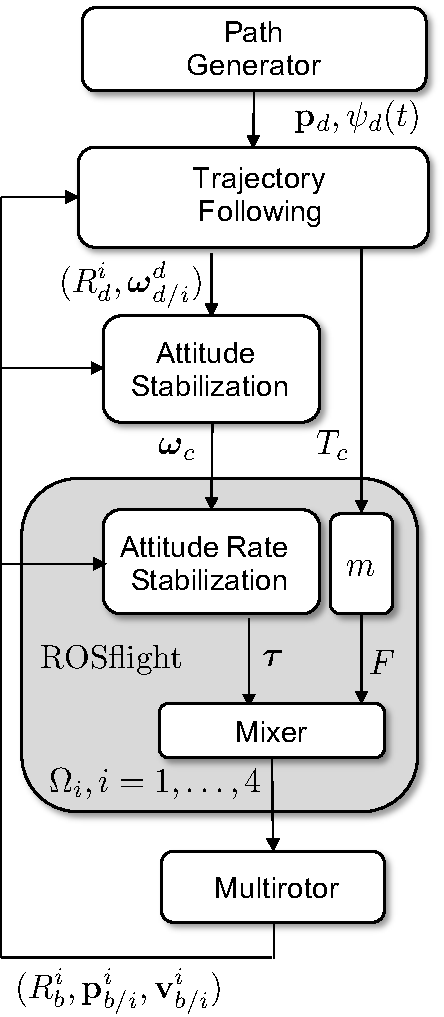
\includegraphics[width=\linewidth]{chap4_trajectory_following/figures/cascaded_trajectory_following}
  \caption{Cascade control architecture for trajectory following.}
  \label{fig:cascaded_trajectory_following}  
\end{marginfigure}
We will assume that the low-level autopilot (labeled ROSflight in Figure~\ref{fig:cascaded_trajectory_following}) implements attitude rate stabilization and accepts a commanded angular velocity $\omegabf_c$, which is the commanded angular velocity of the body relative to the inertial frame, expressed in the body frame, and the commanded throttle $T_c$, which is the commanded force divided by the mass $m$.
The commanded angular rate is supplied by an attitude stabilization loop similar to that derived in Theorem~\ref{thm:attitude_stabilization_rotation_simple}.  
In this section we derive the trajectory following algorithm, where the inputs are the desired inertial position of the multirotor $\pbf_d$, and the desired heading angle $\psi_d$, and their derivatives.

From Equations~\eqref{eq:eom_p}--\eqref{eq:eom_v}, the translational equations of motion are given by
\begin{align}
	\dot{\pbf}_{b/i}^i &= \vbf_{b/i}^i \label{eq:following_pdot_1} \\
	\dot{\vbf}_{b/i}^i &= g \ebf_3 - T_c R_d^i \ebf_3, \label{eq:following_vdot_1}
\end{align}
where we have replaced the throttle $T$ with the commanded throttle $T_c$, and the rotation matrix $R_b^i$ with the desired attitude $R_d^i$, and where we have ignored the induced drag term.
Define the position error as $\tilde{\pbf} \doteq \pbf_{b/i}^i - \pbf_d$, from which we obtain
\begin{equation} \label{eq:cascaded_pddot}
\ddot{\tilde{\pbf}} = g \ebf_3 - T_cR_d^i \ebf_3 - \ddot{\pbf}_d.
\end{equation}

Let the desired rotation matrix be given by
\[
R_d^i = \begin{pmatrix} \rbf_{1d} & \rbf_{2d} & \rbf_{3d} \end{pmatrix},
\]
from which we get
\[
\ddot{\tilde{\pbf}} = g \ebf_3 - T_c\rbf_{3d} - \ddot{\pbf}_d.
\]
The idea behind the trajectory following scheme is to set $T_c\rbf_{3d}$ to achieve PD-like following properties, and then to pick $\rbf_{2d}$ and $\rbf_{1d}$ to align the front of the multirotor with the direction vector
\[
\sbf_{\psi_d} \doteq \begin{pmatrix} \cos\psi_d \\ \sin\psi_d \\  0 \end{pmatrix}.
\]
Toward that end, we have the following scheme.
\begin{theorem}
Given the dynamics in Equation~\eqref{eq:following_pdot_1} and~\eqref{eq:following_vdot_1}, and the desired trajectory given by $\pbf_d(t)$, $\dot{\pbf}_d$, $\ddot{\pbf}_d$, $\psi_d$, $\dot{\psi}_d$, if the throttle and desired rotation matrix are selected as
\begin{align}
T_c &= \norm{\ddot{p}_d - g\ebf_3 - K_p \tilde{\pbf} - K_d\dot{\tilde{\pbf}}} \label{eq:cascaded_attitude_T_c} \\
\rbf_{3d} &= -\frac{\ddot{p}_d - g\ebf_3 - K_p \tilde{\pbf} - K_d\dot{\tilde{\pbf}}}{\norm{\ddot{p}_d - g\ebf_3 - K_p \tilde{\pbf} - K_d\dot{\tilde{\pbf}}}} \label{eq:cascaded_attitude_r_3} \\
\rbf_{2d} &= \frac{\rbf_{3d} \times \sbf_{\psi_d}}{\norm{\rbf_{3d} \times \sbf_{\psi_d}}} \label{eq:cascaded_attitude_r_2}\\
\rbf_{1d} &= \rbf_{2d} \times \rbf_{3d},\label{eq:cascaded_attitude_r_1}
\end{align}
where $K_p=K_p^\top > 0$ and $K_d=K_d^\top > 0$, and where the desired angular velocity is given by
\[
\omegabf_{d/i}^d = (R_d^{i\top}\dot{R}_d^{i})^\vee,
\]
then $\norm{\pbf_{b/i}^i - \pbf_d} \to 0$ and $\psi \to \psi_d$.
\end{theorem}
Note that $R_d^i = (\rbf_{1d}, \rbf_{2d}, \rbf_{3d})$ has been constructed so that the desired body $z$-axis is aligned with the desired acceleration vector, and the body $x$-axis has been aligned so that it is in plane defined by the desired heading direction and the desired acceleration vector.

\begin{proof}
Substituting Equations~\eqref{eq:cascaded_attitude_T_c} and~\eqref{eq:cascaded_attitude_r_3} into Equation~\eqref{eq:cascaded_pddot} gives
\begin{equation} \label{eq:cascaded_pddot}
\ddot{\tilde{\pbf}} = -K_p\tilde{\pbf} - K_d\dot{\tilde{\pbf}}.
\end{equation}
Define the Lyapunov function 
\[
V(\tilde{\pbf},\dot{\tilde{\pbf}}) = \frac{1}{2}\tilde{\pbf}^\top K_p \tilde{\pbf} + \frac{1}{2}\dot{\tilde{\pbf}}^\top \dot{\tilde{\pbf}},
\]
and differentiate to get,
\begin{align*}
\dot{V} &= \dot{\tilde{\pbf}}^\top K_p \tilde{\pbf} + \dot{\tilde{\pbf}}^\top \ddot{\tilde{\pbf}} \\
	&= \dot{\tilde{\pbf}}^\top \left(\ddot{\tilde{\pbf}} + K_p \tilde{\pbf} \right) \\
	&= -\dot{\tilde{\pbf}}^\top K_d \dot{\tilde{\pbf}}.
\end{align*}
Note that if there are no limits on throttle, then $\Omega_c = \{ (\tilde{\pbf}, \dot{\tilde{\pbf}}) ~|~ V \leq c \}$ can be defined by any $c$.  However, if there are throttle limits, then $\Omega_c$ is defined by those limits through Equation~\eqref{eq:cascaded_attitude_T_c}.  
Let 
\[
E=\Omega_c \cap \{(\tilde{\pbf},\dot{\tilde{\pbf}}) ~|~ \dot{V} = 0\} = \Omega_c \cap \{(\tilde{\pbf},\dot{\tilde{\pbf}}) ~|~ \dot{\tilde{\pbf}}\},
\]
and let $M$ be the set of invariant points in $E$.  Then $(\tilde{\pbf},\dot{\tilde{\pbf}})\in M $ implies that $\dot{\tilde{p}}(t)\equiv 0$, where the $\equiv$ symbol is used to mean that the equality holds for all time $t\in (-\infty, \infty)$.  This implies that $\ddot{\tilde{\pbf}}\equiv 0$, which implies from \eqref{eq:cascaded_pddot} that $\tilde{\pbf}\equiv 0$.  Therefore from Theorem~\ref{thm:lasalle_invariance_theorem} $\norm{\tilde{\pbf}}\to 0$.  The attitude stabilization block ensures that $R_b^i(t) \to R_d^i(t)$, and therefore that $\psi(t)\to\psi_d(t)$.
\end{proof}

Additional stuff:

Let 
\[
V=\frac{1}{2}\tilde{\pbf}^\top K_p \tilde{\pbf} + \frac{1}{2}\dot{\tilde{\pbf}}^\top \dot{\tilde{\pbf}}.
\]
Differentiate to get
\begin{align*}
\dot{V} &= \dot{\tilde{\pbf}}^\top \left[ K_p\tilde{\pbf} + g\ebf_3 - TR_b^i\ebf_3 -\ddot{\pbf}_d \right]
\dot{V} &= \dot{\tilde{\pbf}}^\top \left[ K_p\tilde{\pbf} + g\ebf_3 - T\rbf_3 -\ddot{\pbf}_d \right]
\end{align*}
Add and subtract $T\rbf_{3d}/(\rbf_3^\top \rbf_{3d})$ to get
\begin{align*}
\dot{V} &= \dot{\tilde{\pbf}}^\top \left[ K_p\tilde{\pbf} + g\ebf_3 - \frac{T\rbf_{3d}}{(\rbf_3^\top \rbf_{3d})}  -\ddot{\pbf}_d  \left(\frac{(\frac{T\rbf_{3d}}{(\rbf_3^\top \rbf_{3d})})T\rbf_{3}}{(\rbf_3^\top \rbf_{3d})}-\frac{T\rbf_{3d}}{(\rbf_3^\top \rbf_{3d})}\right)\right] \\
&= \dot{\tilde{\pbf}}^\top \left[ K_p\tilde{\pbf} + g\ebf_3 - \frac{T\rbf_{3d}}{(\rbf_3^\top \rbf_{3d})}  -\ddot{\pbf}_d  \left(\frac{T}{(\rbf_3^\top \rbf_{3d})}\right)(I-\rbf_3\rbf_3^\top)\rbf_{3d}\right].
\end{align*}
Now pick
\begin{align*}
\abf_d &= -\ddot{\pbf}_d + g\ebf_3 + K_p\tilde{\pbf} + K_d\dot{\tilde{\pbf}} \\	
\rbf_{3d} &= \frac{\abf_d}{\norm{\abf_d}} \\
T_c &= \abf_d^\top \rbf_3
\end{align*}
resulting in 
\[
\dot{V} = -\dot{\tilde{\pbf}}^\top K_v \dot{\tilde{\pbf}} + \dot{\tilde{\pbf}}^\top (I-\rbf_3\rbf_3^\top )\abf_d.
\]

\rwbcomment{Need to better explain the inner product with $R_b^i \ebf_3$.  Worst case, follow proof of attached paper, but simplify to rotational kinematics.}


%%%%%%%%%%%%%%%%%%%%%%%%%%%%%%%%%%%%%%%%%%%%%%%%%%%%%%%%%%%%%%%
\section{Geometric Tracking Control of a Quadrotor {UAV} on $SE(3)$.}
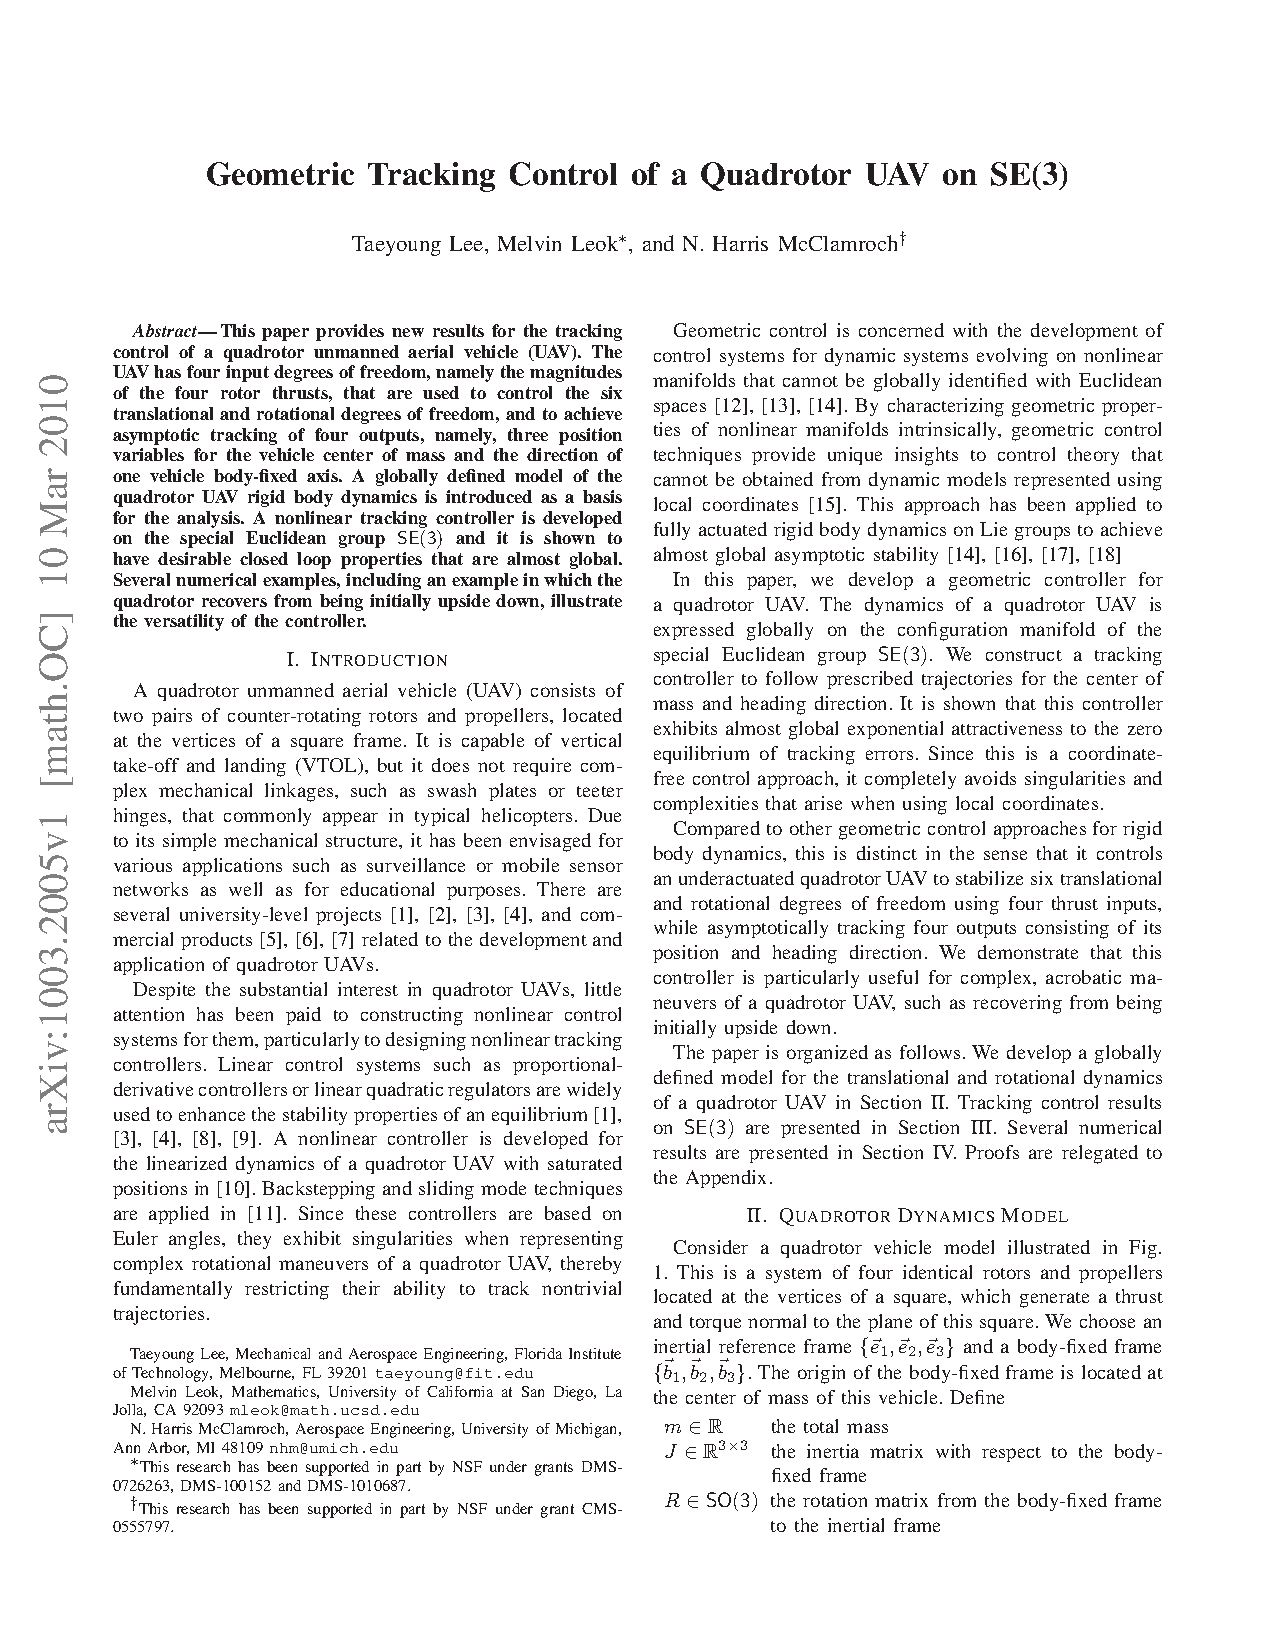
\includepdf[pages=-,scale=.8,pagecommand={}]{chap4_trajectory_following/papers/LeeLeokMcClamroch10_with_proofs.pdf}


%%%%%%%%%%%%%%%%%%%%%%%%%%%%%%%%%%%%%%%%%%%%%%%%%%%%%%%%%%%%%%%
\section{Trajectory following using LQR}

\rwbcomment{develop error state trajectory follower using LQR framework}




